% 翻折 例2：矩形 AB=4 BC=3, 折痕过 D, C 落到 AB 上的 C', BC'=4-√7
\documentclass[tikz,border=4pt]{standalone}
\usepackage{ctex}
\usepackage{amsmath}
\usetikzlibrary{calc}
\begin{document}
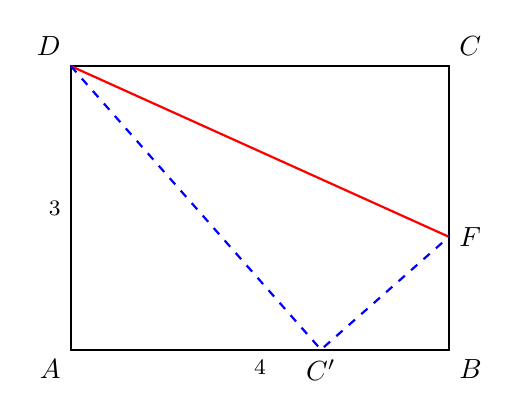
\begin{tikzpicture}[scale=1.2, thick]
  \coordinate (A) at (0,0);
  \coordinate (B) at (4,0);
  \coordinate (C) at (4,3);
  \coordinate (D) at (0,3);
  % C' 在 AB 上, AC' = √7, BC' = 4-√7. C' = (√7, 0)
  \coordinate (Cp) at (2.6458, 0);
  % 折痕过 D, 是 CC' 的中垂线. F 在 BC 上, DF 为折痕
  % CC' 中点 M = ((4+2.6458)/2, 1.5) = (3.3229, 1.5)
  % CC' 方向 = (-1.3542, -3). 垂直方向 (3, -1.3542) 或 (-3, 1.3542)
  % 折痕过 D=(0,3) 且通过 M=(3.3229, 1.5). 验证 D-M = (-3.3229, 1.5), 与 CC' (1.3542,3) 点积 = -3.3229*1.3542+1.5*3 = -4.5+4.5 ≈ 0 ✓
  % F 在 BC 上 (x=4): 直线 D-M 参数 D + t*(M-D), x = 0 + t*3.3229 = 4 -> t = 1.204
  % y = 3 + t*(-1.5) = 3 - 1.806 = 1.194
  \coordinate (F) at (4, 1.194);
  \draw (A)--(B)--(C)--(D)--cycle;
  \draw[red] (D)--(F);
  \draw[blue, dashed] (D)--(Cp)--(F);
  \node[below left] at (A) {$A$};
  \node[below right] at (B) {$B$};
  \node[above right] at (C) {$C$};
  \node[above left] at (D) {$D$};
  \node[below] at (Cp) {$C'$};
  \node[right] at (F) {$F$};
  \node[below] at ($(A)!0.5!(B)$) {\footnotesize $4$};
  \node[left] at ($(A)!0.5!(D)$) {\footnotesize $3$};
\end{tikzpicture}
\end{document}
